\section{Computing concepts}

\begin{frame}
	Computing concepts.
\end{frame}

\begin{frame}
	\frametitle{Hardware}
	\begin{itemize}
		\item Processor.
		\item Memory.
		\item Disc (Input\/Output, I/O).
		\item Graphic User Interface (GUI).
		\item Console, terminal, shell, tty.
		\item Client, server.
	\end{itemize}
\end{frame}

\begin{frame}
	\frametitle{Software}
\end{frame}

\begin{frame}
	\frametitle{Map - Reduce}
	\begin{columns}
		\begin{column}{0.5\textwidth}
			\begin{itemize}
				\item It is a progamming model and its implementation.
				\item It's meant to process large data sets in parallel.
				\item The data sets are distributed on a computer cluster.
				\item Google uses it for processing queries and large dataset of
				      satellite imagery~\cite{dean2008}.
			\end{itemize}
		\end{column}
		\begin{column}{0.5\textwidth}
			\begin{figure}
				\centering
				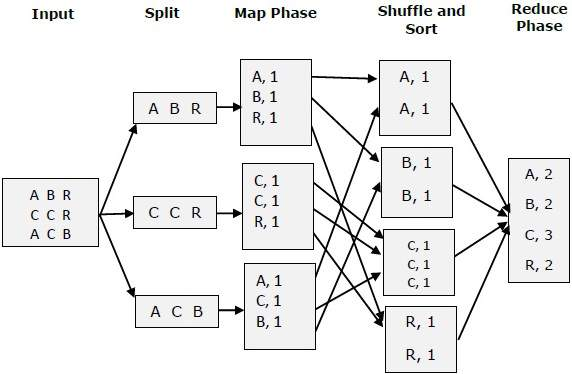
\includegraphics[scale=0.3]
				{img/mapreduce_work.jpg}
				\caption{Source: \href{https://www.tutorialspoint.com/map_reduce/map_reduce_quick_guide.htm}
					{Map reduce quick guide}.}
			\end{figure}
		\end{column}
	\end{columns}
\end{frame}

\begin{frame}
	\frametitle{Databases}
\end{frame}

\begin{frame}
	\frametitle{Resources}
	\begin{columns}
		\begin{column}{0.5\textwidth}
			\begin{itemize}
				\item \href{https://thecrashcourse.com/topic/computerscience/}
				      {Computer Science} by Crash Course.
			\end{itemize}
		\end{column}
		\begin{column}{0.5\textwidth}
			\begin{figure}
				\centering
				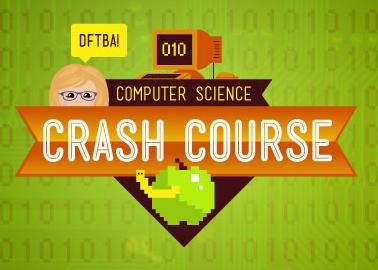
\includegraphics[scale=0.4]
				{img/crash_course_computer_science.jpg}
			\end{figure}
		\end{column}
	\end{columns}
\end{frame}
